\documentclass[10pt]{amsart}
\usepackage[a4paper,margin=22mm]{geometry}
\usepackage{fontspec}
\setmainfont{Latin Modern Roman}[SmallCapsFont={lmromancaps10-regular.otf}]
\usepackage{amsmath,amssymb,amsthm,mathtools,enumitem,hyperref}
\emergencystretch=3em
\newtheorem{proposition}{Proposition}[section]
\newtheorem{claim}[proposition]{Claim}
\newenvironment{enonce*}[2][]{\par\smallskip\noindent\textbf{#2}.\par\nobreak}{\par\smallskip}
\usepackage{tikz, tkz-graph}

\newcommand{\N}{\mathbb{N}}

\usetikzlibrary{arrows}
\newcommand{\vertex}[3]{\node [vertex] (#1) at (#2, #3 * 1.7) {};}
\newcommand{\edge}[2]{\draw (#1) -- (#2);}
\newcommand{\arc}[2]{{\draw[-latex] (#1) edge (#2);}}

\DeclareMathOperator{\im}{im}
\DeclareMathOperator{\Tran}{Tran}
\DeclareMathOperator{\Sing}{Sing}
\DeclareMathOperator{\Sym}{Sym}
\DeclareMathOperator{\Alt}{Alt}
\DeclareMathOperator{\rk}{rk}
\DeclareMathOperator{\id}{id}
\DeclareMathOperator{\Ima}{Im}

\newcommand{\genset}[1]{\langle#1\rangle}
\newcommand{\set}[2]{\{#1:#2\}}

%\newcommand{\LL}{\mathscr{L}}
%\newcommand{\R}{\mathscr{R}}
%\newcommand{\J}{\mathscr{J}}
%\newcommand{\K}{\mathscr{K}}
%\renewcommand{\H}{\mathscr{H}}
\newcommand{\LL}{\mathcal{L}}
\newcommand{\R}{\mathcal{R}}
\newcommand{\J}{\mathcal{J}}
\newcommand{\K}{\mathcal{K}}
\newcommand{\Hcal}{\mathcal{H}}
\newcommand{\easty}[2]{(#1 \to #2)}
\newcommand{\nset}{[n]}



%%%%%%%%%%%%%%%%%%%%%%%%%%%%%%%%%%%%%
\newcommand*{\mk}{\mkern -1mu}
\newcommand*{\Mk}{\mkern -2mu}
\newcommand*{\mK}{\mkern 1mu}
\newcommand*{\MK}{\mkern 2mu}

\hypersetup{urlcolor=purple, linkcolor=blue, citecolor=red}


\newcommand*{\romanenumi}{\renewcommand*{\theenumi}{\roman{enumi}}}
\newcommand*{\Romanenumi}{\renewcommand*{\theenumi}{\Roman{enumi}}}
\newcommand*{\alphenumi}{\renewcommand*{\theenumi}{\alph{enumi}}}
\newcommand*{\Alphenumi}{\renewcommand*{\theenumi}{\Alph{enumi}}}
%%%%%%%%%%%%%%%%%%%%%%%%%%%%%%%%%%


\title[Arc-semigroup cycle length]{Maximum arc-semigroup cycle length for two connected graphs joined at degree-not-one vertices by a long path}
\author{James East; Maximilien Gadouleau; James D. Mitchell}
\date{}
\begin{document}
\maketitle
\noindent\textbf{Source.} Original Proposition 3.6, Structural aspects of semigroups based on digraphs, Algebraic Combinatorics 2 (2019), 711--733, DOI 10.5802/alco.56. Original human proof and required notation follow. The untouched native source and publication are the provenance witnesses.
\section*{Original notation}

A \emph{transformation} of degree $n\in \N$ is a function from $\{1, \ldots,
n\}$ to itself. A \emph{transformation semigroup} is a semigroup consisting
of transformations of equal degree and with the operation of composition of
functions. For the sake of brevity we will denote $\{1,\ldots,n\}$ by $\nset$.
We define $(a \to b)$ to be the transformation defined by
\begin{equation*} 
v (a \to b) = 
 \begin{cases}
 b & \text{if } v = a\\
 v & \text{otherwise}
 \end{cases} 
\end{equation*}
where $a, b \in \nset$ and $a \ne b$. A \emph{digraph} is an ordered pair
$(V, A)$, where $V$ is a set whose elements are referred to as
\emph{vertices}, and $A\subseteq (V\times V) \setminus \{(v,v) : v \in V\}$
is a set of ordered pairs called
\emph{arcs}. We identify a transformation $(a \to b)$ with an arc $(a, b)$
in a digraph and we refer to $(a \to b)$ as an arc. If $D$ is a digraph,
we denote by $\langle D \rangle$ the semigroup generated by
the arcs of $D$, and we refer to such a semigroup as \emph{arc-generated}.

If $A$ is empty, then $D$ is an empty digraph, and $\genset{D}$ is the empty
semigroup. Because this is a degenerate case, and in order to simplify the
statement of our results, we shall always assume that $D$ is not empty (and
hence, that $\genset{D}$ is not the empty semigroup). 

Unless otherwise stated, the vertex set of
a digraph will be $\nset$ for some $n\in \N$. 

The \emph{in-degree} of a vertex $v$ in a digraph $D$ is the number of arcs
of the form $(u, v)$ in $D$; similarly, the \emph{out-degree} of $v$ is the
number of arcs of the form $(v, u)$ in $D$. A vertex $v$ in a digraph $D$ is
called a \emph{sink} if the out-degree of $v$ is $0$. A vertex is
\emph{isolated} if it has no incoming or outgoing arcs. 

If $D = (V, A)$ is a digraph, and $U$ is subset of the vertices $V$ of $D$,
then the \emph{subdigraph of $D$ induced by $U$} is the digraph with vertices
$U$ and arcs $A \cap (U\times U)$. In general, a \emph{subdigraph} of $D =
(V,A)$ is any digraph $D' = (V', A')$ with $V' \subseteq V$ and $A' \subseteq
A\cap (V' \times V')$.

A \emph{walk} in a digraph is a finite sequence $(v_0, v_1, \ldots,
v_r)$, $r\geq 1$, of vertices such that $(v_i, v_{i + 1})$ is an arc for all
$i\in \{0, \ldots, r - 1\}$; the \emph{length} of this walk is $r$. A
\emph{path} is a walk where all vertices are distinct. A \emph{cycle} in a
digraph is a walk where $v_0 = v_r$ and all other vertices are distinct.
A digraph is called \emph{acyclic} if it has no cycles.

A \emph{graph} $G$ is defined to be a digraph where $(u, v)$ is an arc if and
only if $(v, u)$ is an arc in $G$. We refer to the pair of arcs above as the
\emph{edge} $\{u, v\}$. Vertices $u$ and $v$ of a graph $G$ are
\emph{adjacent} if $\{u, v\}$ is an edge of $G$. 

An induced subdigraph of a graph, is also a graph, which we refer to as an
\emph{induced subgraph}. A \emph{spanning subgraph} (as opposed to an
induced subgraph) of a graph $G = (V, A)$ is any graph $H = (V, B)$ where $B
\subseteq A$. 

The \emph{degree} of a vertex in a graph is its in-degree, which equals
its out-degree. If $u$ and $v$ are vertices of a graph $G$, then the
\emph{distance} from $u$ to $v$ is the length of a shortest path from $u$ to
$v$, if such a path exists.

We denote by $K_n$ the \emph{complete graph} with vertices $\nset$
and edges $\{u,v\}$ for all distinct $u,v \in \nset$; by $K_{k, 1}$
the \emph{star graph} with vertices $\{1, \ldots, k + 1\}$ and edges
$\{i, k + 1\}$ for all $i \in \{1, \ldots, k\}$. We denote by $P_n$ the
\emph{path graph}, or simply \emph{path} if there is no ambiguity, with vertices
$\nset$ and edges $\{i, i + 1\}$ for all $i \in \{1, \ldots, n-
1\}$. We denote by $C_n$ the \emph{cycle graph} with vertices $\{1, \ldots,
n\}$ and edges $\{1, n\}$ and $\{i, i + 1\}$ for all $i \in \{1, \ldots, n-
1\}$.

We denote by $\Tran_n$ the monoid consisting of all of the transformations of
degree $n$ where $n\in \N$; called the \emph{full transformation monoid}.
This monoid plays the same role in semigroup theory as the symmetric group does
in group theory, in that every finite semigroup is isomorphic to a subsemigroup
of some $\Tran_n$. Green's relations on $\Tran_n$ can be described in terms of
the following natural parameters associated to transformations. The
\emph{image} of a transformation $\alpha\in \Tran_n$ is the set
\[\im(\alpha)=\set{x\alpha}{x\in\{1, \ldots, n\}};\]
the \emph{kernel} of $\alpha$ is the equivalence relation
\[\ker(\alpha)=\set{(x,y)\in\{1, \ldots, n\}\times\{1, \ldots,
n\}}{x\alpha=y\alpha};\]
and the \emph{rank} of $\alpha$ is
\[\rk(\alpha)=|\im(\alpha)|.\]


A \emph{cycle} of length $k$ in $\alpha\in \Tran_n$ is a sequence of distinct
points $a_0, a_1, \dots, a_{k-1}\in\nset$ such that $a_i \alpha = a_{i+1}$ for
all $i$, where the indices are computed modulo $k$. This section is concerned
with cycles of transformations in an arc-generated semigroup. In particular,

The length of a longest cycle of $\alpha$ is denoted as $l(\alpha)$ and for a
digraph $D$ we write
\[l(D) = \max \{ l(\alpha) : \alpha \in \genset{D} \}.\]
\setcounter{figure}{1}
The next result concerns connected graphs that can be decomposed into two
connected induced subgraphs with a path connecting them. With this in mind, we
introduce a construction based on paths. Let $L$ and $R$ be two connected
graphs on $m$ and $s$ vertices, respectively, where $m \le s$, and let~$P$ be a
path with $q$ vertices. Let $L \oplus_q R$ denote the graph obtained by adding
an edge between an endpoint of $P$ and a vertex of $L$ of degree not equal to
1, and an edge between the other endpoint of $P$ to a vertex of $R$ of degree
not equal to 1. Even though this definition depends on the choice of
attachment vertices, we will omit them in the notation, for our purpose is to
derive results that do not depend on them, apart from the fact that they do not
have degree 1 in $L$ and $R$. We remark that $m, s \ne 2$, since the only
connected graph on two vertices is $K_2$, whose vertices both have degree 1.
However, it is possible to have $m=1$ or $s=1$.

The vertices of $R$ are denoted as $r_1, \dots, r_s$, where they are sorted in
weakly increasing order of distance to the path $P$. In particular, $r_1$ is
attached to $P$, and $r_2$ and $r_3$ are neighbours of $r_1$ if $s\not=1$. A
similar notation is used for $L$; in particular $l_1$ is attached to $P$. Write
$L^* = L \setminus \{ l_1 \}$, $R^* = R \setminus \{ r_1 \}$, $P^* = P \cup
\{l_1, r_1\}$, and order the elements of the path as $p_1, \dots, p_q$ so that
$p_1$ is adjacent to $l_1$, and $p_q$ is adjacent to $r_1$; finally, we also
write $l_1 = p_0$ and $r_1 = p_{q+1}$. For instance, the graph $K_{3,1}
\oplus_4 C_4$ is illustrated in Figure~\ref{fig:oplus}.

\begin{figure}[ht]
\centering
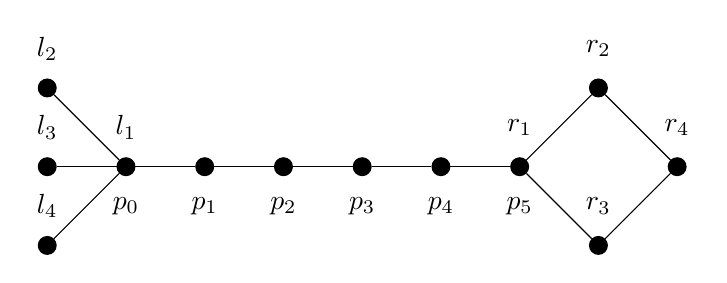
\begin{tikzpicture}[vertex/.style={circle, 
 draw, 
 fill=black,
 inner sep=0.08cm}]
	\node [vertex] (l1) at (1,1) {};
	\node [vertex] (l2) at (0,2) {};
	\node [vertex] (l3) at (0,1) {};
	\node [vertex] (l4) at (0,0) {};

	\node (ll1) at (1,1.5) {$l_1$};
	\node (ll2) at (0,2.5) {$l_2$};
	\node (ll3) at (0,1.5) {$l_3$};
	\node (ll4) at (0,0.5) {$l_4$};
	\node (pp0) at (1,0.5) {$p_0$};

	\node [vertex] (p1) at (2,1) {};
	\node [vertex] (p2) at (3,1) {};
	\node [vertex] (p3) at (4,1) {};
	\node [vertex] (p4) at (5,1) {};

	\node (pp1) at (2,0.5) {$p_1$};
	\node (pp2) at (3,0.5) {$p_2$};
	\node (pp3) at (4,0.5) {$p_3$};
	\node (pp4) at (5,0.5) {$p_4$};

	\node [vertex] (r1) at (6,1) {};
	\node [vertex] (r2) at (7,2) {};
	\node [vertex] (r3) at (8,1) {};
	\node [vertex] (r4) at (7,0) {};

	\node (rr1) at (6,1.5) {$r_1$};
	\node (rr2) at (7,2.5) {$r_2$};
	\node (rr3) at (8,1.5) {$r_4$};
	\node (rr4) at (7,0.5) {$r_3$};
	\node (pp5) at (6,0.5) {$p_5$};
	
 \edge{l1}{l2}
 \edge{l1}{l3}

 \edge{l1}{l4}

 \edge{l1}{p1}
 \edge{p1}{p2}
 \edge{p2}{p3}
 \edge{p3}{p4}
 \edge{p4}{r1}

 \edge{r1}{r2}
 \edge{r2}{r3}
 \edge{r3}{r4}
 \edge{r4}{r1}
\end{tikzpicture}
\caption{The graph $K_{3,1} \oplus_4 C_4$.} \label{fig:oplus}
\end{figure}

\setcounter{section}{3}\setcounter{proposition}{5}
\begin{proposition}[cf. Theorem 1(5)(b) in~\cite{Horvath2017aa}] \label{prop:L+R}
 With the above notation, if $q \ge s$, then 
 \[
 l(L \oplus_q R) = \begin{cases}
 1 &\text{if } m = s = 1\\
 s - 1 &\text{if } m = 1, s \ge 3\\
 m + s - 3 & \text{otherwise.}
 \end{cases}
 \]
\end{proposition}
\begin{proof}
 We write $G = L \oplus_q R$. If $m=s=1$, then $G = P_n$ where $n = q+2$, and
 hence $\genset{P_n}$ is the semigroup of order-preserving transformations
~\cite{Aizenshtat1962aa}, which is aperiodic. Otherwise, we have $s \ge 3$ and we view the
 result as two matching upper and lower bounds on $l(G)$.
 %\medskip

\begin{enonce*}[remark]{Lower bound} 
 Throughout this part of the proof, if $u, w_1, \ldots, w_t, v$ is a path in
 $G$, then we define \[(u\rightsquigarrow v)=(u\to w_1)(w_1\to
 w_2)\cdots(w_{t-1}\to w_t)(w_t\to v)\in\genset G.\] Since this transformation
 depends on the choice of path, we will always specify the path. 
 %\medskip
\end{enonce*} 
 
\begin{enonce*}[remark]{Case 1: ${m = 1}$}
 We will show that there exists $\alpha \in \genset{G}$ containing the cycle
 $r_2, \dots, r_s$. 

 For each $3 \le i \le s$, we choose $r'_i\in \{r_2, r_3\}$ such that there
 is a shortest-length path from $r_1$ to $r_i$ that avoids $r'_i$. We also
 define
 \begin{itemize}
 \item 
 $(r_2 \rightsquigarrow p_2)$ to follow 
 the path $r_2, r_1, p_q, \ldots, p_2$,

 \item 
 $(p_{j - 1} \rightsquigarrow r_j)$ to follow a shortest-length path
 avoiding $r_j'$ and $(r_j\rightsquigarrow p_j)$ to follow the reverse of
 such a path (but omitting the last edge) for all $3 \leq j \leq s$,

 \item
 $(r'_j \rightsquigarrow r'_{j - 1}) = (r'_j \to r_1) (r_1 \to r'_{j -
 1})$ for all $4 \leq j \leq s$, even if $r'_j=r'_{j-1}$,

 \item
 $(r_s \rightsquigarrow r'_s)$ to follow any path avoiding vertices from
 $P$.
 \end{itemize}
 It is straightforward to verify that 
 \[
 \alpha = \left[
 \prod_{i = 2}^{s - 1} 
 (r_i \rightsquigarrow p_i)
 \right]
 \cdot 
 (r_s \rightsquigarrow r'_s) 
 \cdot 
 \left[
 \prod_{j = s} ^ {4} 
 (p_{j-1} \rightsquigarrow r_j)
 (r'_j \rightsquigarrow r'_{j-1}) 
 \right] 
 \cdot 
 (p_2 \rightsquigarrow r_3) \in\genset{G}
 \]
 contains the cycle $r_2, \dots, r_s$, as required (the second
 product is computed in descending order of the indices). We also note that
 $l_1\alpha=l_1$.
\end{enonce*}
% \medskip

\begin{enonce*}[remark]{Case 2: ${m \geq 3}$}
 As in Case 1, we may use $K_1 \oplus_q R\subseteq G$ to create
 $\alpha\in\genset{G}$ containing the cycle $r_2, \ldots, r_s$ and such that
 $l_i\alpha = l_i$ for all $i$. Similarly, we may use $L\oplus_q
 K_1\subseteq G$ to create $\beta\in\genset{G}$ containing the cycle
 $l_2, \ldots, l_m$ and such that $r_i\beta = r_i$ for all $i$. If 
 $(r_2 \rightsquigarrow l_3)$ and $(l_2
 \rightsquigarrow r_2)$ follow the unique shortest paths, then 
 $\gamma = \alpha \beta (r_2 \rightsquigarrow l_3) (l_2 \rightsquigarrow
 r_2)\in\genset{G}$ contains the cycle $l_3, \ldots, l_m, r_2, \ldots, r_s$.
\end{enonce*}
% \medskip

\begin{enonce*}[remark]{Upper bound} 
Since $l(G_1) \le l(G_2)$ if $G_1$ is a subgraph of $G_2$, we assume without
loss of generality that $G = K_m \oplus_q K_s$. 
We define a pre-order $\preceq$ on the vertices of $G$ such that 
$a \preceq b$ if $a \in L ^*$, or $b \in R ^ *$, or $a = p_i$ and $b= p_j$ for some
$0\leq i\leq j\leq q+1$. If $a\preceq b$ and $b\not\preceq a$, then we write
$a \prec b$ or $b\succ a$. We note that $b\not\preceq a$ implies $a\preceq b$. 
We define the sets
\[a^+ = \{b \in \nset : b \succ a \} \cup \{a\}\quad\text{and}\quad
a^- = \{b \in \nset : a \succ b \} \cup \{a\}.\]
For the remainder of the proof, we fix some $\gamma\in\genset{G}$, and we write $\gamma
= \epsilon_1 \cdots \epsilon_k$, where $\epsilon_1, \ldots, \epsilon_k$ are arcs
in $G$. We also define $\gamma_0 = \id$ and $\gamma_i = \epsilon_1 \cdots
\epsilon_i$ for all $1 \le i \le k$.
%\medskip
\end{enonce*}

\begin{enonce*}[remark]{Case 1: ${m = 1}$}
We require the following claim.
\end{enonce*}

\begin{claim} \label{claim:jumping1}
 Suppose that $m = 1$. If there are vertices $u$ and $v$ in $G$ such that
 $u\preceq v$ and $u\gamma \succ v\gamma$, then $\gamma \in \alpha \genset{G}$
 for some $\alpha \in \genset{G} \cup \{ \id \}$ such that $u^+ \alpha
 \subseteq R^*$.
\end{claim}

\begin{proof}
 If $u \in R^*$, then $u^+=\{u\}$ and so $\alpha = \id$ has the required
 properties. Suppose that $u \notin R^*$. Since $u \gamma \succ v \gamma$,
 there exists $i$ such that $u \gamma_i \in R ^ *$. If $j$ is the least such
 value, then $u \gamma_{j-1} = r_1$, $u^+ \gamma_{j-1} \subseteq R$, and
 $\epsilon_j = (r_1 \to r_a)$ for some $r_a \in R^*$. If we set $\alpha =
 \gamma_j$, then $u^+ \alpha = (u^+ \gamma_{j-1})\epsilon_j \subseteq R^*$.
\end{proof}

Seeking a contradiction, suppose that $\gamma$ has
a cycle of length $c$, where $c \geq s$, and let $C = \{u_1, \dots, u_c\}$
be such a cycle, where $u_1 \preceq\cdots\preceq u_c$. It is
not necessarily the case that $u_i \gamma = u_{i+1}$. Since $|C| = c > s - 1 =
|R ^ *|$, $C$ is not contained in $R^*$ and so $u_1 \prec u_i$ for all $i \ne 1$. 
%
This gives $C\subseteq u_1^+$.
%
Let $j$ be such that $u_j\gamma=u_1$. Then $u_1\prec u_j$ but $u_1\gamma\succ u_j\gamma$.
%
So by Claim~\ref{claim:jumping1}, $c = |C \gamma|
\le |u_1^+ \gamma| \le |R^*|=s-1$, which is the desired contradiction. 
%\medskip
%\end{enonce*}

\begin{enonce*}[remark]{Case 2: ${m \geq 3}$}
For the sake of obtaining a contradiction, suppose that $\gamma$ has a cycle of length at least $m + s - 2$. Let $C =
\{u_1, \dots, u_c\}$ be such a cycle, sorted so
that $u_1 \preceq \cdots\preceq u_c$. Again it is not
necessarily the case that $u_i \gamma = u_{i+1}$. We note that $u_c \notin L$
(since $c \ge m+1$) and $u_1 \notin R$ (since $c \ge s+1$), whence $u_c \succ
u_1$. 

We say that a vertex $v$ of $G$ is of
\emph{$L$-type} if there is $\beta \in \genset{G} \cup \{ \id \}$ such that
$\gamma \in \beta \genset{G}$ and $v^- \beta \subseteq L^*$. Similarly, we
say that $v$ is of \emph{$R$-type} if there is $\alpha \in \genset{G} \cup
\{ \id \}$ such that $\gamma \in \alpha \genset{G}$ and $v^+ \alpha \subseteq
R^*$. 
\end{enonce*}

\begin{claim} \label{claim:jumping2}
 Suppose that $m\ge 3$. If there are vertices $u$ and $v$ in $G$ such that
 $u\preceq v$ and $u\gamma \succ v\gamma$, then either
 $u$ is of $R$-type, or $v$ is of $L$-type.
\end{claim}
\begin{proof} 
 As in the proof of Claim~\ref{claim:jumping1}, if $u \in R^*$, then 
 $\alpha = \id$ witnesses that $u$ is of $R$-type. Similarly, if 
 $v \in L^*$ then $\beta = \id$ shows that $v$ is of $L$-type. 
 
 Suppose that $u \notin R^*$ and $v \notin L^*$. As before, for some $i\in
 \{1, \ldots, k\}$, $u\gamma_i$ and $v\gamma_i$ both belong to $L^*$ or
 $R^*$. Suppose that both $u\gamma_i$ and $v\gamma_i$ belong to $R^ *$ before
 they both belong to $L ^ *$; the case when they both first belong to $L^*$ is
 symmetric. Let $i$ be the least value such that $u\gamma_i, v\gamma_i\in R ^
 *$. Then for all $j < i$, $u\gamma_j \preceq v\gamma_j$ and either
 $u\gamma_j \notin R^*$ or $v\gamma_j \notin R^*$. If $u\gamma_j \in R ^*$
 for some $j < i$, then since $u\gamma_j\preceq v\gamma_j$, it follows that
 $v\gamma_j \in R ^*$. Hence $i$ is the least value such that $u\gamma_i\in
 R ^ *$.

 We will show that $u\gamma_j \not\in L^*$ for all $0 \leq j < i$. Seeking a
 contradiction, suppose that $u\gamma_j\in L^*$ for some $0\leq j < i$, and
 let $b = \max\{j : j < i,\ u\gamma_j \in L^*\}$. The vertices $\nset$ of $G$ can be partitioned into two parts:
 \[A = (\{u\gamma_b\} \cup
 P^* \cup R^*) \gamma_b^{-1} \qquad\text{and}\qquad B
 = (L^* \setminus \{u\gamma_b\}) \gamma_b^{-1}.\]
 Let $x \in A$. If $x \gamma_b = u \gamma_b$, then $x \gamma_i = u \gamma_i
 \in R^*$. Otherwise, $u \gamma_b \prec x \gamma_b$.
 %
 By maximality of $b$ and minimality of $i$, we have $\epsilon_{b+1}=(u\gamma_b\to l_1)$, $\epsilon_i=(r_1\to u\gamma_i)$, $u\gamma_j\in P^*$ for all $b<j<i$, and $u\gamma_j\preceq x\gamma_j$ for all $b<j<i$. It follows that $x\gamma_i\in R^*$.
%
 Therefore, $A\gamma_i \subseteq R ^*$, and so 
 \[c \le \rk(\gamma) \le |B \gamma_b| + |A \gamma_i| \le (m-2) + (s-1) = m + s
 - 3,\]
 which contradicts the fact that $c > m+s-3$. 

 We conclude that $u\gamma_j \in P^*$ for all $j < i$, and by the argument
 concluding the proof of Claim~\ref{claim:jumping1}, we obtain $u^+\gamma_i
 \subseteq R^*$, so that $u$ is of $R$-type.
\end{proof} 


\begin{claim} \label{claim:jump}
 There exist $u, v \in C$ such that $u\preceq v$, $u_c\preceq v$, and $u\gamma
 \succ v\gamma$. There also exist $u', v' \in C$ such that $u'\preceq v'$,
 $u' \preceq u_1$, and $u'\gamma \succ v'\gamma$. 
\end{claim}

\begin{proof}
 If $u_c \in R^*$, then since $C$ intersects $R^*$ but is not contained in
 $R^*$, there exist $u, v \in C$ such that $u \notin R^*$, $u \gamma \in
 R^*$, $v \in R^*$, and $v \gamma \notin R^*$. Then $u$ and $v$ have the
 required properties.

 If $u_c \notin R^*$, then $u_c \succ u_i$ for all $1 \le i \le c-1$. In
 particular, if $u_c=u_j\gamma$, then $u = u_j$ and $v = u_c$ have the
 required properties.

The proof of the existence of $u'$ and $v'$ is symmetrical.
\end{proof}

We now write $X = \set{u_i \in C}{\exists j,\ u_i\preceq u_j,\ u_i\gamma \succ
u_j\gamma}$, and note that $X\not=\varnothing$ by Claim~\ref{claim:jump}.
%
We enumerate $X = \{x_1, \dots, x_d\}$ such that $x_1 \preceq\cdots\preceq x_d$. For each $1\leq i\leq d$,
let $y_i$ be an element of $C$ such that $x_i\preceq y_i$ and $x_i\gamma
\succ y_i\gamma$; we also assume that $y_i$ is maximal with respect to this property: that is, if $v\in C$ is such that $x_i\preceq v$ and $x_i\gamma \succ v\gamma$,
then $v \preceq y_i$. Note that $\{y_1, \ldots, y_d\}$ is not necessarily
sorted according to the pre-order. If $y_M$ is a maximal element of $\{y_1,
\ldots, y_d\}$ with respect to $\preceq$, then Claim~\ref{claim:jump} indicates
that $u_c \preceq y_M$. We also have $x_1 \preceq u_1$, since $x_1\preceq u'$, where $u'$ is as in Claim \ref{claim:jump}.

%We now determine a crucial property of $X$. 
\begin{claim} \label{claim:jumping3}
 There exists $1 \le a < d$ such that $y_1, \dots, y_a$ are all of $L$-type
 and $x_{a+1}, \dots, x_d$ are all of $R$-type. Moreover, for all $i > a \ge
 j$, $x_i \succ y_j$.
\end{claim}

\begin{proof} 
 We shall prove a sequence of facts about the set $X$, the last two of which give the claim.
 %\medskip

\begin{enumerate}[label=(\alph*)]
 \item\label{proof_claim3.10_a} 
 If $x_i$ is of $R$-type, and if $x_i \preceq y_j$, then $y_j$
 is not of $L$-type.
 %\medskip

 %\noindent 
 Suppose to the contrary that we have the following: $x_i \preceq
 y_j$; $\alpha, \beta \in \genset{G} \cup \{ \id \}$; $\gamma \in \alpha
 \genset{G}$ and $\gamma \in \beta \genset{G}$; $x_i^+ \alpha \subseteq R^*$
 and $y_j^- \beta \subseteq L^*$. We then have $x_i \notin L^*$, for otherwise
 $\nset = L^* \cup x_i^+$ and \[ c \le \rk(\gamma) \le |L^*
 \setminus \{ x_i \}| + |x_i^+ \alpha| \le (m-2) + (s-1) = m + s - 3, \] a
 contradiction. Similarly, we have $y_j \notin R^*$. Thus 
 \[ x_i, y_j \in P^*, \quad \nset = x_i^+ \cup y_j^-, \quad x_i \in
 x_i^+ \cap y_j^-. \] 
 Denoting $S = \{ w \in y_j^- : w \gamma= x_i \gamma \}$, we have \[ c \le
 \rk(\gamma) \le |(x_i^+ \cup S) \gamma| + |(y_j^- \setminus S) \gamma| \Mk =\Mk 
 |x_i^+ \gamma| + |y_j^- \gamma| - 1 \le (s-1) + (m-1) - 1 = m + s - 3, \] a
 contradiction.
% \medskip

% \textbf{(b).} 
 \item\label{proof_claim3.10_b} 
 For every $i$, $x_i$ is of $R$-type if and only if $y_i$ is not of $L$-type.
 %\medskip

% \noindent 
Apply~\ref{proof_claim3.10_a} with $i=j$ and combine with Claim~\ref{claim:jumping2}.
% \medskip

 \item\label{proof_claim3.10_c} 
 % \textbf{(c).} 
 If $x_i$ is of $R$-type, then so too are $x_{i+1},\ldots,x_d$.
% \medskip

% \noindent 
If $x_i$ is of $R$-type and $i < j$, then because $x_i\preceq x_j\preceq y_j$, \ref{proof_claim3.10_a}~says that $y_j$ is not of $L$-type and~\ref{proof_claim3.10_b} in turn says that $x_j$ is of $R$-type.
% \medskip

% \textbf{(d).} 
\item\label{proof_claim3.10_d}
$y_1$ is of $L$-type and $x_M$ is of $R$-type.
% \medskip

% \noindent 
 We prove that $x_1$ is not of $R$-type, which by~\ref{proof_claim3.10_b} implies that $y_1$ is of $L$-type. Suppose that $x_1^+ \alpha \subseteq R^*$ for some
 $\alpha\in\genset{G}\cup\{\id\}$ with $\gamma\in\alpha\genset{G}$. If $x_1 \in
 L^*$, then $x_1^+ = \{x_1\} \cup P^* \cup R^*$ and hence 
 \[ 
 c \le \rk(\gamma)
 \le |L^* \setminus \{x_1\}| + |(\{x_1\} \cup P^* \cup R^*)\alpha| \le (m-2) +
 (s-1) = m + s - 3 ,
 \]
  a contradiction. If $x_1 \notin L^*$, then $x_1 = u_1$
 (since $x_1 \preceq u_1$ and $u_1 \not\in R^*$) and hence $C \subseteq x_1^+$, so
 that $c=|C\gamma| \le |x_1^+ \alpha| \le s-1$, a contradiction. The proof for $x_M$ is
 symmetrical.
 %\medskip

% \textbf{(e).} 
 \item\label{proof_claim3.10_e} 
 There exists $1 \le a < d$ such that $y_1, \dots, y_a$ are all of
 $L$-type and $x_{a+1}, \dots, x_d$ are all of $R$-type.
% \medskip

 This follows from combining~\ref{proof_claim3.10_b}, \ref{proof_claim3.10_c} and~\ref{proof_claim3.10_d}, with 
 \[
 a\Mk =\Mk \max\set{i\Mk }{\Mk y_1,\ldots,y_i \text{ are of $L$-type}}.
 \]
% \medskip

 \item\label{proof_claim3.10_f}  
 %\textbf{(f).} 
 For all $i > a \ge j$, $x_i \succ y_j$.
% \medskip

 By~\ref{proof_claim3.10_e}, $x_i$ is of $R$-type, and $y_j$ of $L$-type. It follows from~\ref{proof_claim3.10_a} that 
 \[
 x_i \succ y_j.\qedhere
\]
\end{enumerate}
\end{proof}

We now partition $C$ into two parts $A$ and $B$ defined by
\[A = \{ u \in C : x_{a+1} \succ u \} \qquad\text{and}\qquad
B = \{ v \in C : x_{a+1} \preceq v \}.\]
Note that $A$ and $B$ are both non-empty: for example, $x_{a+1}\in B$ and $y_a\in A$.
Since $C$ is a cycle of $\gamma$, $S \gamma \ne S$ for any non-empty proper 
subset $S$ of $C$. In particular, $A \gamma \ne A$ and $B \gamma \ne B$, and so 
there exist $u\in A$ and $v\in B$ such that $u \gamma \in B$ and $v \gamma \in A$.
It follows that $u\preceq v$ and $u\gamma \succ v\gamma$, and hence
$u = x_j$ and $v \preceq y_j$ for some $j \le
a$. But then $x_{a+1}\preceq v\preceq y_j$, which
contradicts Claim~\ref{claim:jumping3}.
\end{proof}
\begin{thebibliography}{11}
\bibitem[1]{Aizenshtat1962aa} A. Ya. A\u{\i}zenshtat, The defining relations of the endomorphism semigroup of a finite linearly ordered set, Sib. Mat. Zh. 3 (1962), 161--169.
\bibitem[11]{Horvath2017aa} Gábor Horváth, Chrystopher L. Nehaniv, and Károly Podoski, The maximal subgroups and the complexity of the flow semigroup of finite (di)graphs, International Journal of Algebra and Computation 27 (2017), no. 7, 863--886.
\end{thebibliography}
\end{document}
